\newpage

\begin{appendices}
  \section{Quantitative Research – Survey} \label{appendix:quantitative}
  
    \begin{figure}[H]
      \centering
      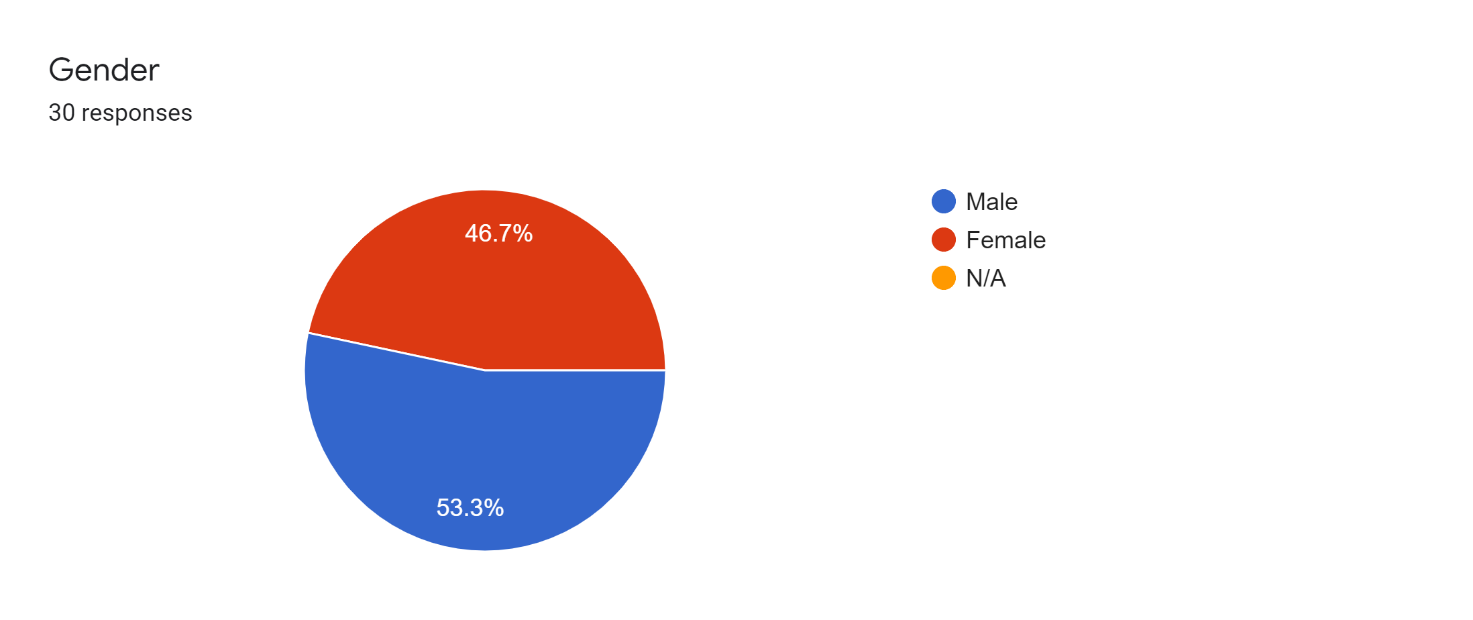
\includegraphics[width=18cm]{img/Survey/Q1.png}
      % \caption*{#3}
    \end{figure}
    \begin{figure}[H]
      \centering
      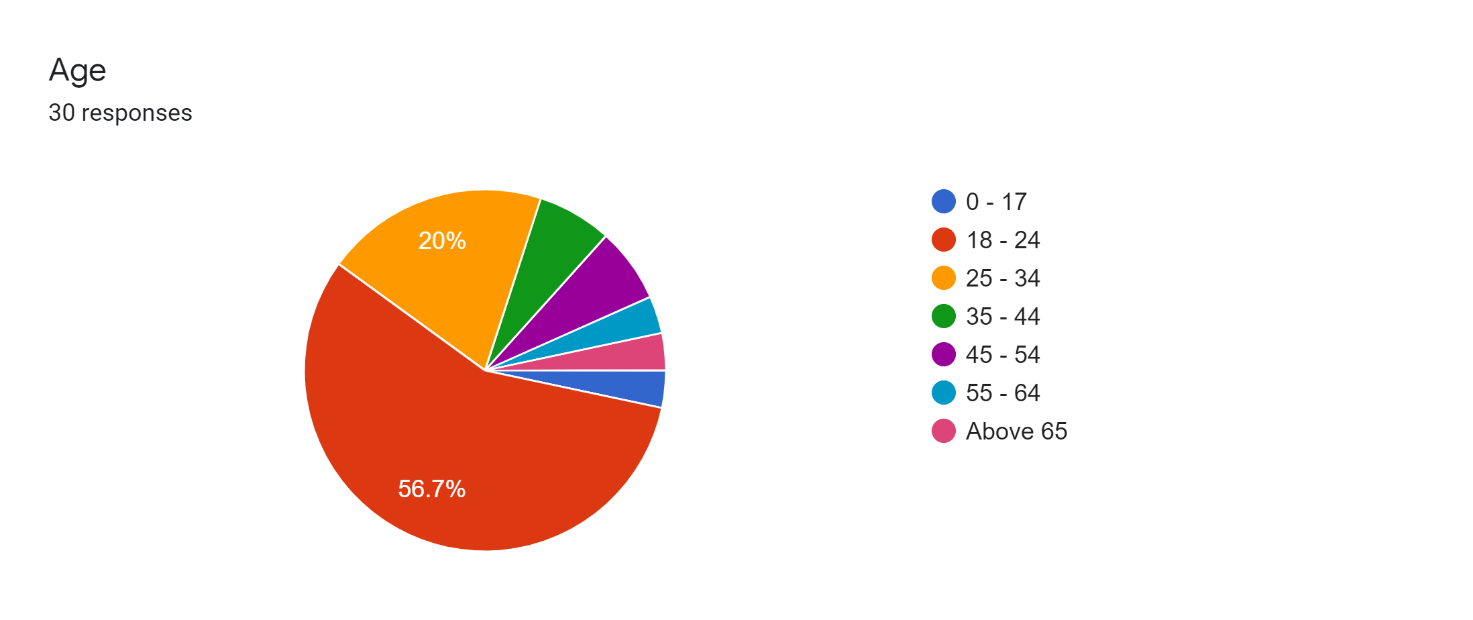
\includegraphics[width=18cm]{img/Survey/Q2.png}
      % \caption*{#3}
    \end{figure}
    \begin{figure}[H]
      \centering
      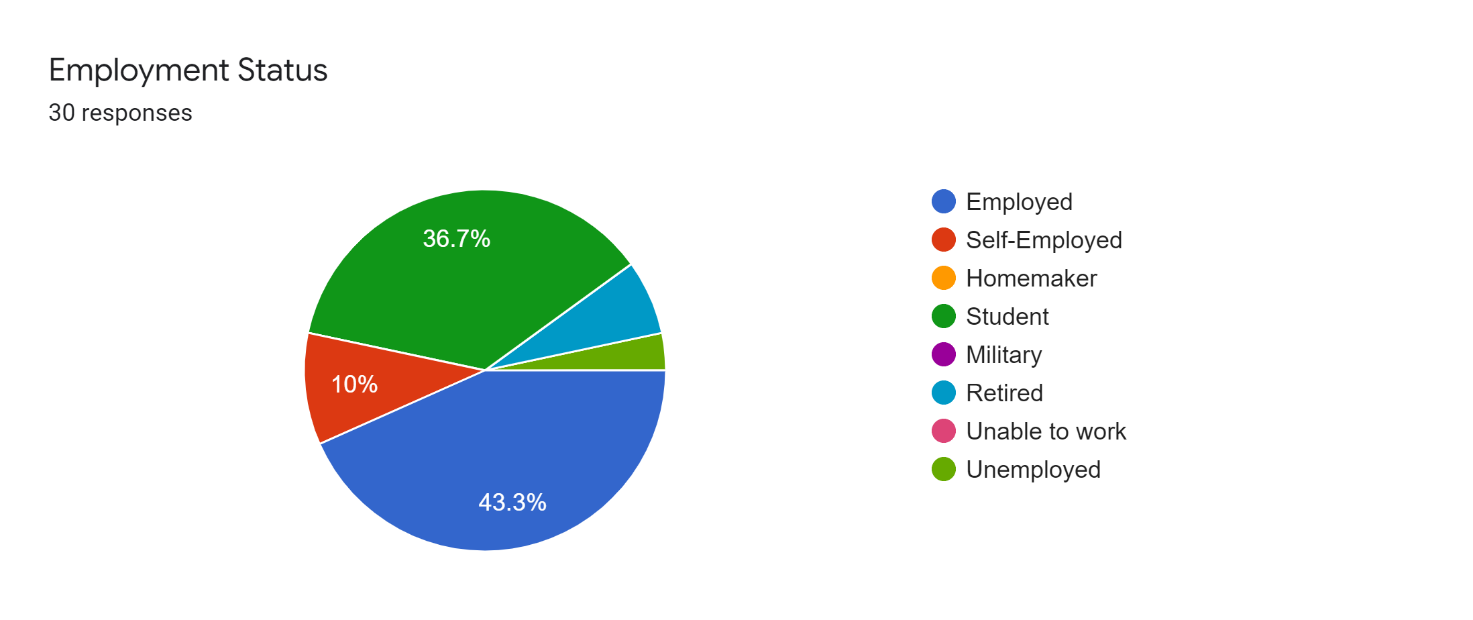
\includegraphics[width=18cm]{img/Survey/Q3.png}
      % \caption*{#3}
    \end{figure}
    \begin{figure}[H]
      \centering
      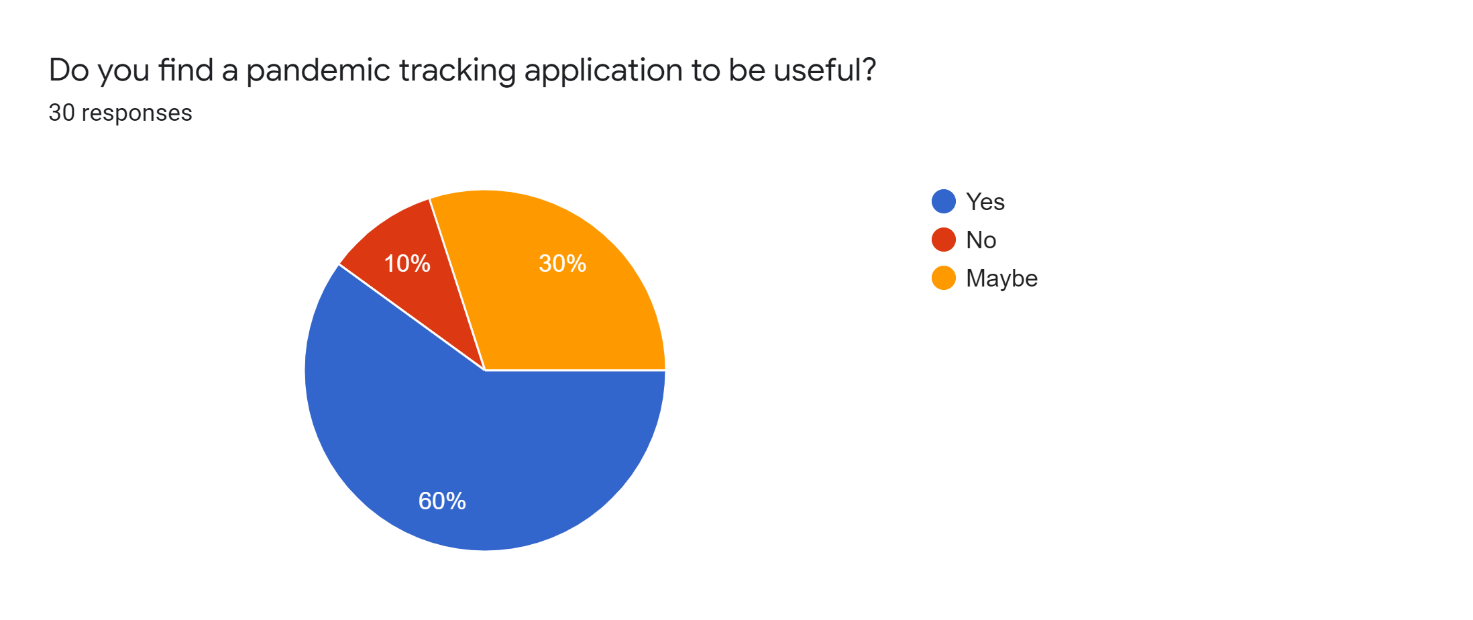
\includegraphics[width=18cm]{img/Survey/Q4.png}
      % \caption*{#3}
    \end{figure}
    \begin{figure}[H]
      \centering
      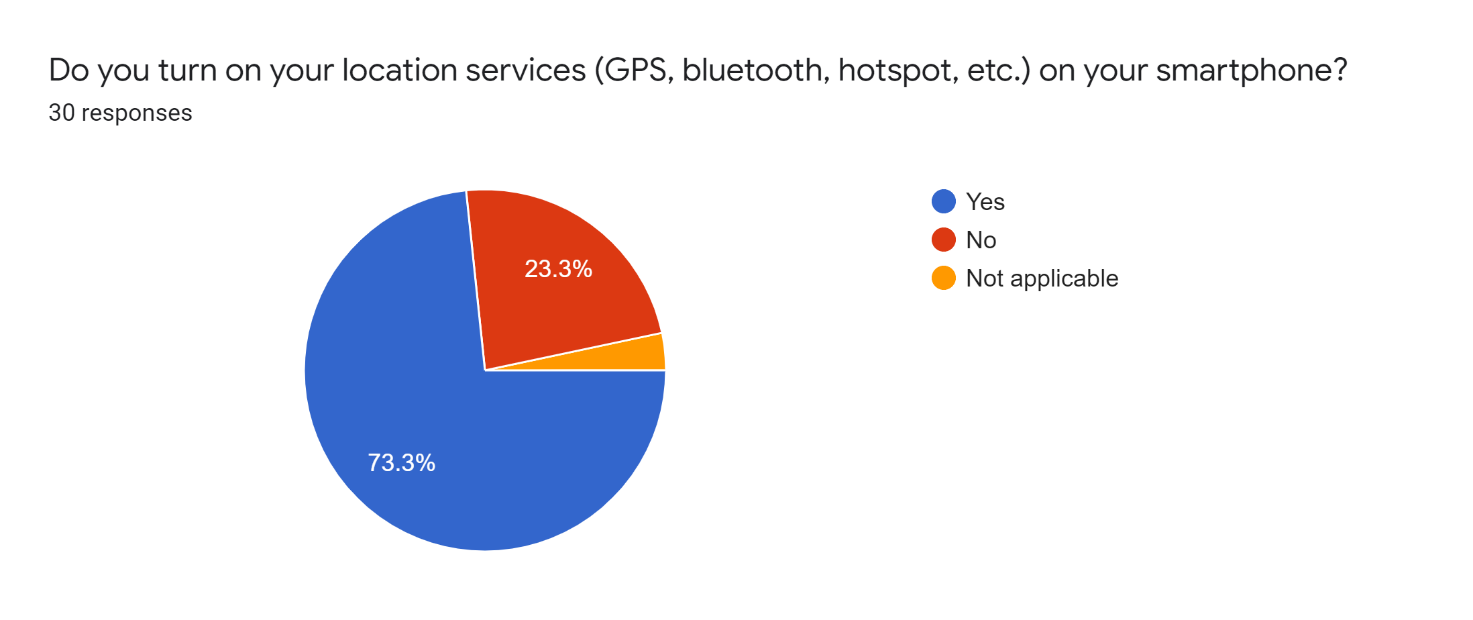
\includegraphics[width=18cm]{img/Survey/Q5.png}
      % \caption*{#3}
    \end{figure}
    \begin{figure}[H]
      \centering
      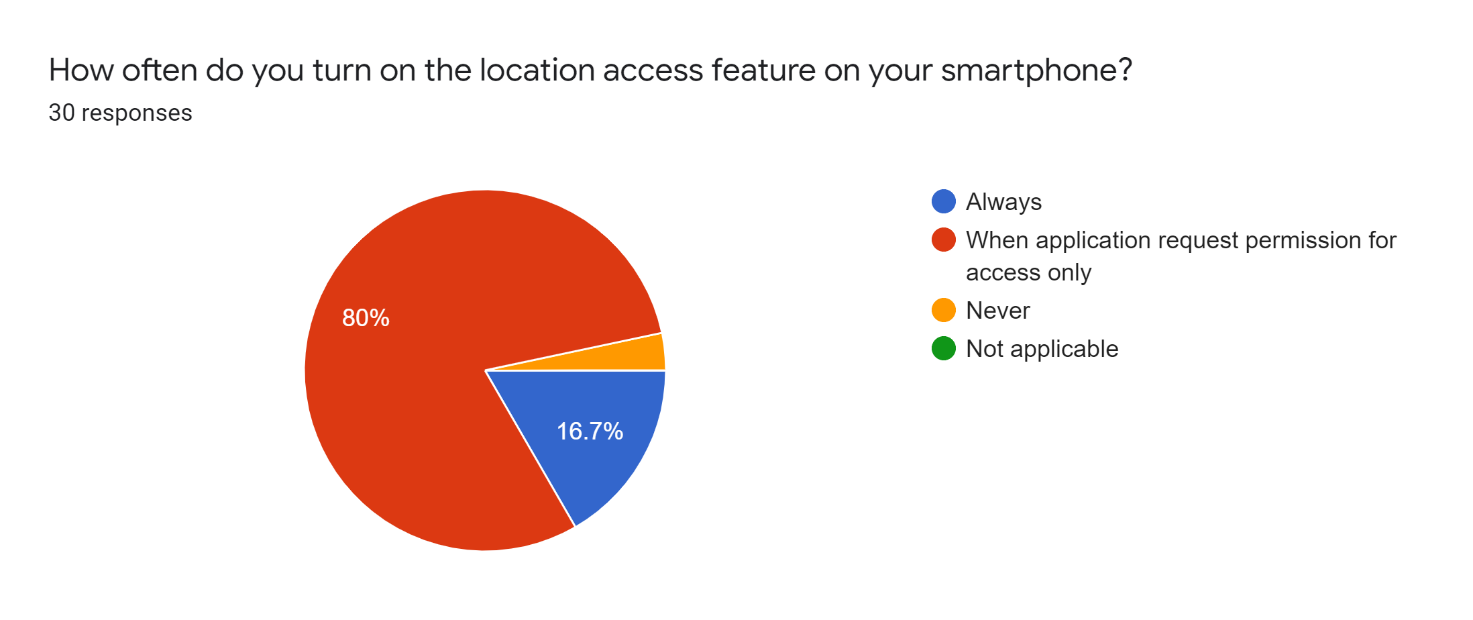
\includegraphics[width=18cm]{img/Survey/Q6.png}
      % \caption*{#3}
    \end{figure}
    \begin{figure}[H]
      \centering
      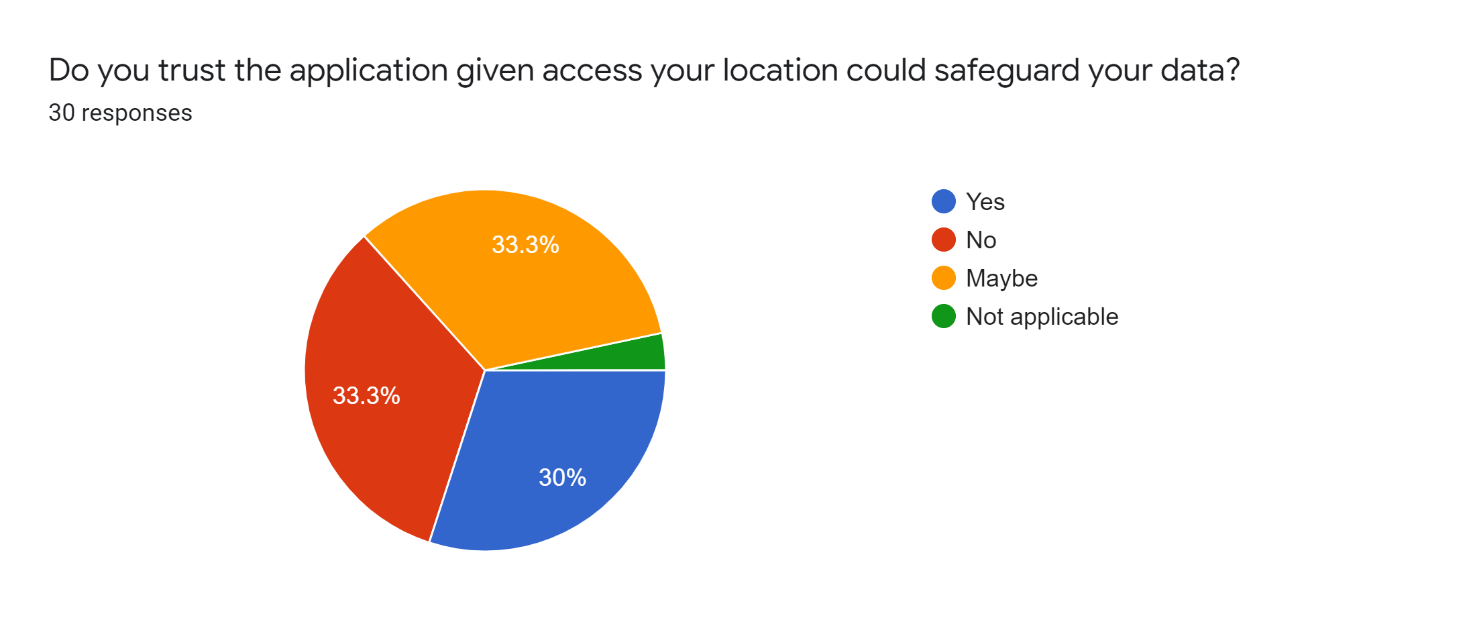
\includegraphics[width=18cm]{img/Survey/Q7.png}
      % \caption*{#3}
    \end{figure}
    \begin{figure}[H]
      \centering
      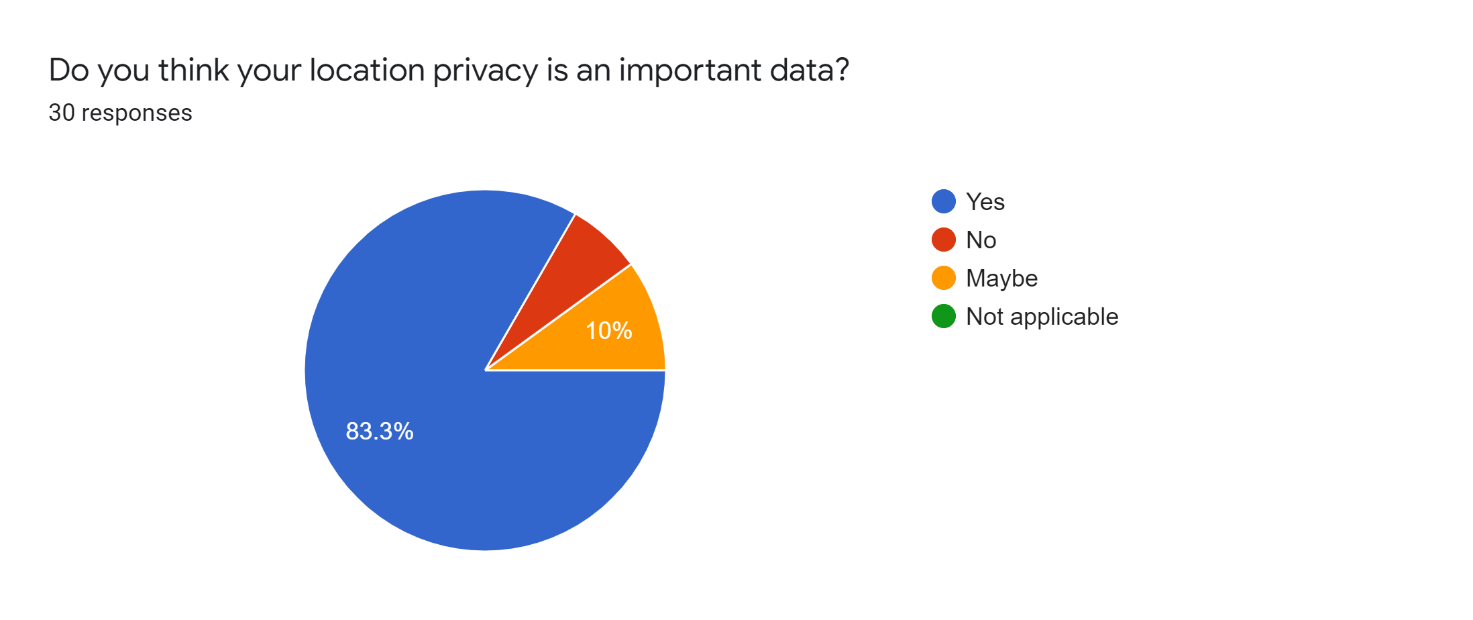
\includegraphics[width=18cm]{img/Survey/Q8.png}
      % \caption*{#3}
    \end{figure}
    \begin{figure}[H]
      \centering
      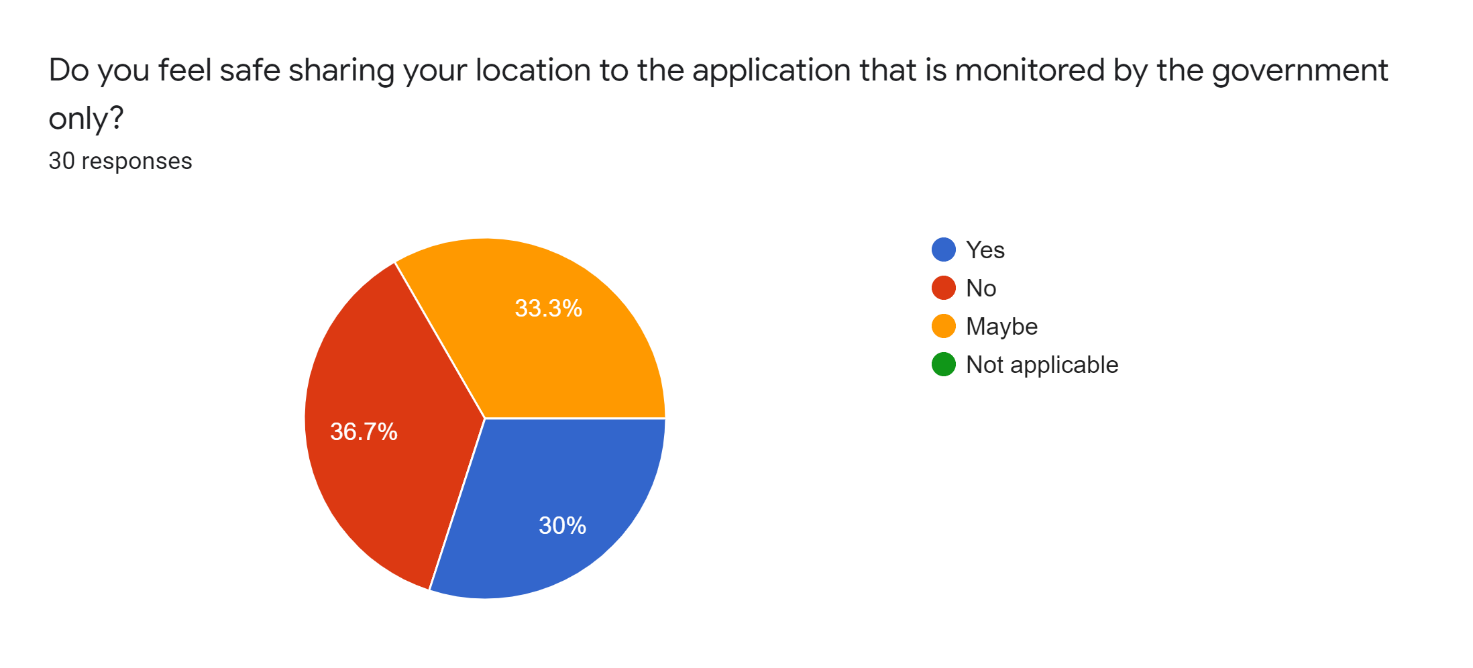
\includegraphics[width=18cm]{img/Survey/Q9.png}
      % \caption*{#3}
    \end{figure}

  \section{Qualitative Research - Interview} \label{appendix:qualitative}

    \subsection{Interview 1 Transcript (Primary School Student)}
      \begin{itemize}
        \item \textbf{Interviewer}: A
        \item \textbf{Interviewee \#1}: B
      \end{itemize}
      \par \textit{Answers are slightly modified for clarity purposes}

      \begin{itemize}
        \item A: Hi “B”, do you want your parents to accompany you during this session?
        \item B: Nope, I’m all good.
        \item A: OK, let’s start straight away.
        \item A: With the current pandemic situation in Australia, how do you find yourself coping with it?
        \item B: I am staying safe at home most of times. As my classes will be moved to a home-based
  learning on Term 2 onwards, my parents will want me to be a little more motivated in my
  studies. As I never done this before, I find myself a little scare especially not being able to
  play with my mates.
        \item A: Do you think the government is handling the current pandemic situation well?
        \item B: I’m not very sure how the government is responding to this situation, but I think some
  measures should be taken at an earlier stage when patients number are still low.
        \item A: Based on the data collection from my survey, around 60% of my respondents think that a
  pandemic tracking application is useful. What do you think?
        \item B: I think it would be more useful for my parents as they need to go outdoors for essential
  activities. As a kid of my age, I spent most of time at home like other of my mates as well. So,
  I think listening to my parents to stay at home would be safe enough without needing this
  application. My mates also told me that their parents do not allow them to join in groceries
  shopping as well. That is why I don’t think I need it since I’m listening to what my parents
  tell me. Also, I am not interested in knowing these things.
        \item A: Ok, let me end with one last question. Please tell me if you do not understand my question.
        \item B: Ok.
        \item A: Do you think your parents telling the government their real-time location through the
  smartphone is good or bad thing for safety purposes?
        \item B: As long as the government can keep my parents safe. If not, I think it is useless.
        \item A: What do you mean by that?
        \item B: I know from my mate that my parents sharing their location could also put me in risk as well
  if the data is not handled well, which I believe the government should be responsible for taking
  care my parents data, if not removing it.
        \item A: I think you are tired as well now. Thank you so much for your time. See you soon.
        \item B: Cheers.
      \end{itemize}

      \subsection{Interview 2 Transcript (Retail Worker)}
      \begin{itemize}
        \item \textbf{Interviewer}: A
        \item \textbf{Interviewee \#2}: C
      \end{itemize}
      \par \textit{Answers are slightly modified for clarity purposes}

      \begin{itemize}
        \item A: Morning “C”, are you prepared?
        \item C: Yes, let’s go.
        \item A: With the current pandemic situation in Australia, how do you find yourself coping with it?
        \item C: Well, I am currently rostered with a maximum of a 10 hours shift weekly, which I have been
        reduced to a quarter of my normal weekly shift hours. It’s kind of frustrating as I have
        mortgage and other commitments. I would say it is very tough for me during this period.
        \item A: Despite your reduced shift hours, I assume that you are still not thinking to stop temporarily
        with this ongoing pandemic situation?
        \item C: I would say it’s on a horn of a dilemma, I understand it’s between wealth or health, but I do
        not have a ticket for both sides, which is why I still choose to pay my bills.
        \item A: Besides that, do you think the government is handling the current pandemic situation well?
        \item C: I don’t think the government is enforcing enough restrictions on the movement control of the
        people. I believe it needs a more comprehensive strategy to monitor all the people that
        currently resides in Australia under this kind of situation.
        \item A: Following up on your response, how do you see a pandemic tracking application?
        \item C: It’s a good concept that can be made feasible. But I still have doubts with the government
        collecting my location data.
        \item A: So, what do you think can go wrong?
        \item C: I believed that our location data are considered personal information, which should be our
        user privacy as a fundamental rights. I think that the government needs a system that could
        prevent data breaches to allow the users feel safe giving consent to share this piece of
        information for all legal and valid purposes.
        \item A: For example, if a kind of security mechanism is used to safeguard the data, do you feel more
        confident in sharing the location data?
        \item C: I’m not tech savvy but I know there is no security system that is unbreachable now. I believe
        if the government could least create a top-tier security system, I would be joining as a user.
        \item A: I think that is all for me. I appreciate your valuable time and input for my further research.
        \item C: No worries, catch you later.
      \end{itemize}
  
    \subsection{Interview 3 Transcript (Retired Elderly)}
      \begin{itemize}
        \item \textbf{Interviewer}: A
        \item \textbf{Interviewee \#3}: D
      \end{itemize}
      \par \textit{Answers are slightly modified for clarity purposes}

      \begin{itemize}
        \item A: Hi “D”, how are you feeling today?
        \item D: Same as usual.
        \item A: So why not let us get this interview done and you could enjoy the rest of the day?
        \item D: I’ll be glad.
        \item A: Firstly, how do you find yourself coping with this current pandemic situation in Australia?
        \item D: I’m still alive and kicking but still very anxious when going out grabbing some essentials
        sometimes as you won’t know how well this fragile and vulnerable body could withstand.
        \item A: No worries “D”. I believe good hygienic practices could reduce the risk of being infected.
        Please don’t hesitate to contact me with any shopping if you need a helping hand.
        \item D: Nah, my kids would help me from time to time to stock up so no worries.
        \item A: Alright, so do you think the government is handling the current pandemic situation well?
        \item D: In terms on the restrictions and measures, there is still space for improvement to reduce the
        spread rate. As for caregiving support, I believe the government and other bodies have been
        doing well to support this community group of taking care of our wellbeing. My folks also
        told me that the government is close collaborating with NGO parties to prioritize medical
        support for our community. I am quite satisfied.
        \item A: How about the necessity of a pandemic tracking application then?
        \item D: I believed it would not be very convenient for an old folk like me and others. As I started
        experiencing functional loss on different aspects of my body following my days, I find
        difficulties in using digital devices other than calling someone now.
        \item A: I understand. If the application has a simple and friendly user interface, or even technology
        that assist disabilities. Do you think it will be more accepting in your community group?
        \item D: If additional support is provided in any form that could help us to understand the application.
        It would serve as a huge boost for older folks like us to use it. Count me in!
        \item A: Lastly, my research on a recent survey show that one-third of the respondents could trust the
        application with protecting the data, another one-third of not able to protect the data, and the
        remaining of having doubts with the application safeguarding the data respectively. So, what
        do you think about the data protection on an application?
        \item D: As much I am concerned with the data protection scheme of the application, I believe
        everything has a risk, nevertheless for this pandemic tracking application too. So, a method to
        earn the peoples’ trust is to formulate a best possible strategy that could mitigate to a minimum
        impact as much as possible.
        \item A: Thank you so much for your precious time and valuable input. Have a good day and take care.
        \item D: It’s my pleasure. See you.
      \end{itemize}

\end{appendices}